\documentclass[a4paper]{article}
\usepackage[utf8]{inputenc} %Unicode UFT-8 symbols.
\usepackage{amsmath} %three dots
\usepackage{graphicx} %insert figures
\usepackage[danish]{babel} %dansk¨
\usepackage{hyperref} % links cliclable


\title{Boblesortering}
\author{Roar Nind Steffensen \& Asger Græsholt}
\date{\today}


\begin{document}

\maketitle

\begin{abstract}
    Dette dokument omhandler boblesortering. Der beskrives algoritmen og præsenteres en kompleksitetsanalyse.
\end{abstract}


\section{Introduktion}

Boblesortering (\textit{eng. bubble sort}) er en populær \textit{sorteringsalgoritme} og er en af de simpleste algoritmer at forstå og implementere. Dog er den ikke en særlig effektiv sorteringsalgoritme\footnote{Mere om dette i “Algoritmer og Datastrukturer 1”} ; hverken for store eller små lister, og den anvendes sjældent i praksis. Boblesortering sorterer, som navnet antyder, elementerne i en liste ved at \textit{boble} hvert element gennem listen til sin rette plads i listen.

\subsection{Pseudokode}

Wikipedia~\cite{wiki} giver følgende pseudokode for boblesortering.

\begin{verbatim}
procedure bubbleSort( A : list of sortable items ) defined as:
  do
    swapped := false
    for each i in 0 to length(A) - 2 inclusive do:
      if A[i] > A[i+1] then
        swap( A[i], A[i+1] )
        swapped := true
      end if
    end for
  while swapped
end procedure
\end{verbatim}
En illustration af en kørsel af boblesortering fra Wikipedia kan ses på figur \ref{fig:bubblesorting}.

\section{Analyse af boblesortering}
Antallet af sammenligninger, som boblesortering udfører på en tabel af længde $n$, er i værste fald

\begin{equation*}
    \sum_{i=1}^{n-1} i = 1 + 2 + 3 + \dotsb + n - 1 = \frac{n(n-1)}{2}.
\end{equation*}

I bedste fald er antallet $n-1$. Se tabel \ref{tab:vb}.

\begin{figure}[h!]
    \centering
    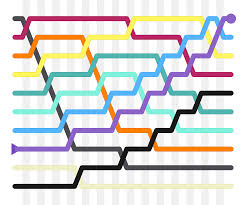
\includegraphics[width=7cm]{bs.jpeg}
    \caption{Illustration af boblesortering.}
    \label{fig:bubblesorting}
\end{figure}

\begin{table}[h!]
    \centering
        \begin{tabular}{|l|l|}
            \hline
            \textbf{Værst} & $n(n-1)/2$ \\ \hline
            \textbf{Bedst} & $n-1$ \\ \hline
        \end{tabular}
    \caption{Antal sammenligninger for boblesortering}
    \label{tab:vb}
\end{table}

\section{Videre læsning}
For en komplet introduktion til boblesortering og relaterede sorteringsalgoritmer se Knuth~\cite{ComArt}.

\begin{thebibliography}{99}
\bibitem{ComArt}Donald Knuth. The Art of Computer Programming, Volume~3. Addison-Wesley.
\bibitem{wiki} \url{http://en.wikipedia.org/wiki/Bubble\_sort}
\end{thebibliography}

\end{document}
